\section{AI segmentation task}
\textbf{Test some of the AI segmentation plugins to segment the same anatomical structures: } \\

Using the newest data processment tools has been created plugins to work with models. Concretely the artificial intelligence has been used to develop those plugins. A good example is the plugin that will be used in this exercise: Total Segmentator. Those plugins are created and shared by medical engineers from universitys, for example the one that is used has been created by the Research and Analysis team of the Research Hospital in Basel. The pluguin consists on a tool for segmentation of most major anatomical structure in any CT or MR image. The tool was trained on a wide range of different CT and MR (different scanners, institutions, protocols…) and therefore works well on most images. \\

The steps to use the plugin are the following:

\subsection{}
Enter to the Total Segmentator module and select the input button as can be seen in the \textbf{\textit{\cref{fig:ai_step1}}}
\begin{figure}[H]
    \centering
    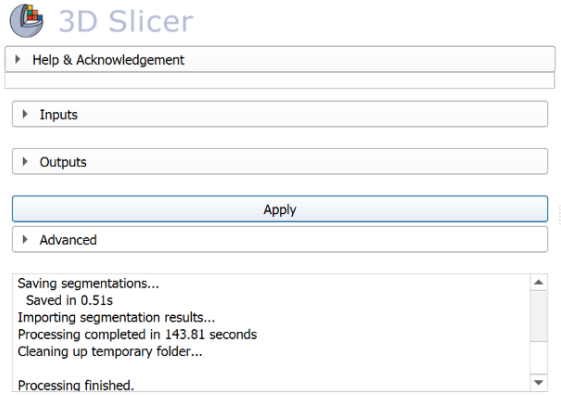
\includegraphics[width=0.7\textwidth]{img/ex53.png}
    \caption{Initial menu of the Total Segmentation plugin tool.}
    \label{fig:ai_step1}
\end{figure}


\subsection{}
In the input part of the menu will be necessary to select the 3D model which is used, in this case the CTChest as it is visible in the input volume. It is necessary also to select the segmentation task that is required, it is possible to to segmentate different parts of the data alone or all the parts at the same time. As it is not possible to segmentate the lungs and the thoracic bones at the same time it has been chosen to segmentate all the parts. 
This plugin can work with extreme precision since is using a powerful tool of segmentation. The drawback of it is that it requires a high performance laptop to run it and approximately one hour of computer work. Since the computer used to do it is not powerful enough, the Fast option has been selected. This option runs a fast version of the plugin without the level of detail that can perform but in a really lower time. The computer used lasted 10 minutes to obtain as a result the image of the 
\textbf{\textit{\cref{fig:ai_result}}}.

\begin{figure}[H]
    \centering
    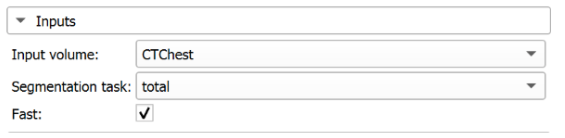
\includegraphics[width=0.7\textwidth]{img/ex54.png}
    \caption{Option menu of the Total Segmentation plugin tool.}
    \label{fig:ai_step2}
\end{figure}

\begin{figure}
    \centering
    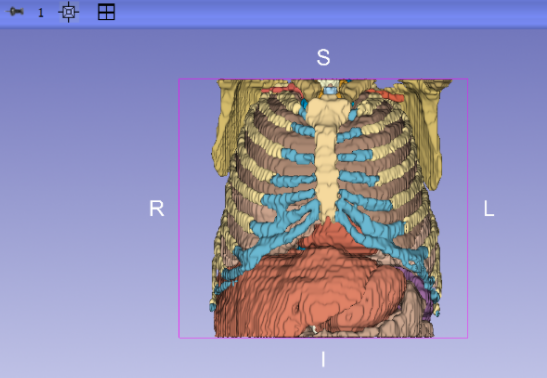
\includegraphics[width=0.7\textwidth]{img/ex55.png}
    \caption{First result of the usage of the Total Segmentation plugin tool in the CTChest data.}
    \label{fig:ai_result}
\end{figure}

Finally by selecting the visualize or not visualize option in the segment editor for the segments that we are not interested in as it is visible in the Fig~\ref{fig:ai_step2}, it is possible to achieve the final segmentation of the lung and the thoracic bones with a regular precision as it is visible in the Fig~\ref{fig:ai_result}.

\begin{figure}[H]
    \centering
    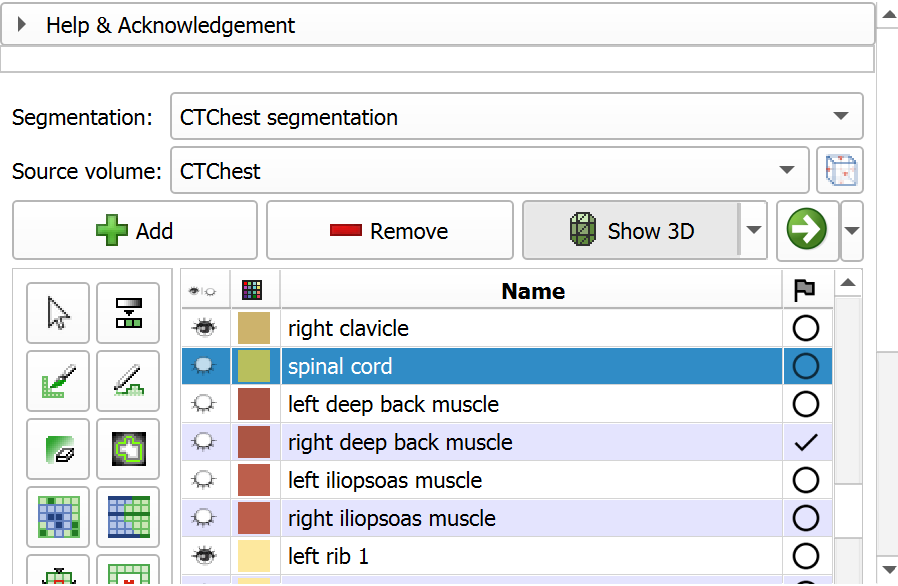
\includegraphics[width=0.7\textwidth]{img/ex51.png}
    \caption{List of segmentation created by the IA tool and selection of the visualization option for the segments that are of our interest.}
    \label{fig:ai_final_result}
\end{figure}

\begin{figure}[H]
    \centering
    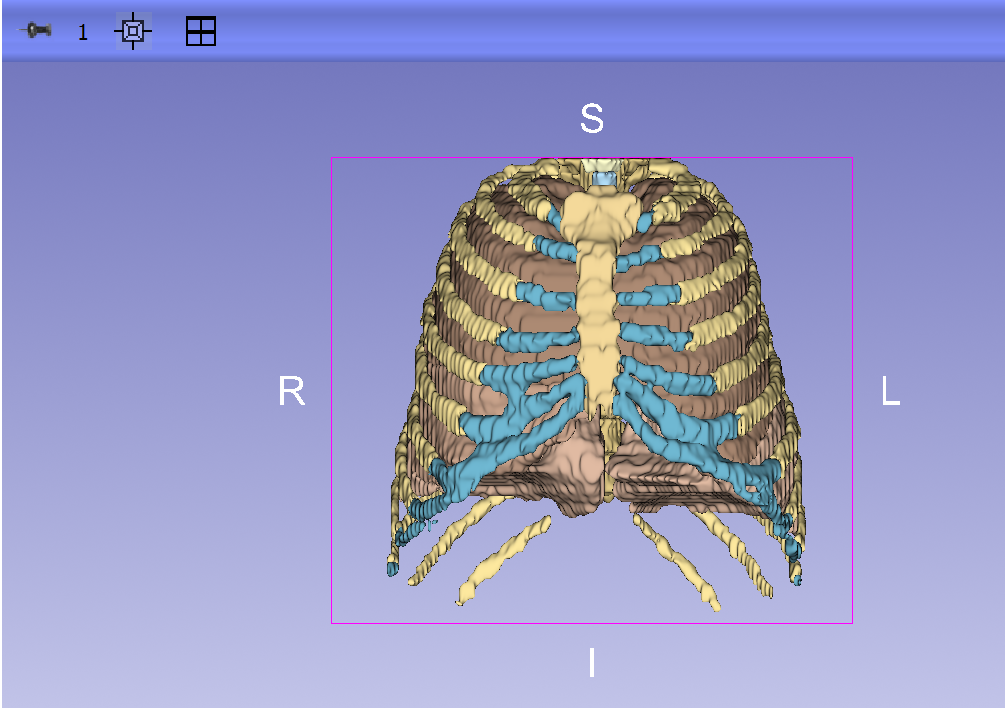
\includegraphics[width=0.7\textwidth]{img/ex52.png}
    \caption{Final figure of the segmentation of the lungs and thoracic bones.}
    \label{fig:ai_final_result2}
\end{figure}

\begin{itemize}
    \item Is it possible to use some IA module to obtain the same result? 
    \item If not, which is the closer approximation that you can obtain automatically? 
    \item From the obtained approximation, could it be possible to achieve the same result using the Segment Editor module? 
    \item Explain how (it is not necessary to compute the segmentation, just only explain the procedure to follow).
\end{itemize}

So, finally yes, it is possible to use an IA module to obtain the same result that the obtained before, in fact if with this plugin we would haven’t used the fast option in the menu, we would have obtained better results than now or better that the obtained by classical segmentation methods. \\

It is possible to obtain the same results using only the tools that provide the Segment Editor module because it is similar to the way that this plugin works, by creating precise segmentation segments. The drawback is that to do this work it would be necessary to use a lot of time on segmentation work instead of the one hour of work that the plugin needs to obtain a precise segmentation result. \\

The procedure to follow to obtain the same result using the segment editor module will be based on the tools explained on the first exercise: the threshold segmentation, the scissors segmentation and the island segmentation.  
